\begin{abstract}
	Hard parameter sharing for multi-task learning is widely used in empirical research despite the fact that its generalization properties have not been well established in many cases. This paper studies its generalization properties in a fundamental setting: How does hard parameter sharing work given multiple linear regression tasks? We develop new techniques and establish a number of new results in the high-dimensional setting, where the sample size and feature dimension increase at a fixed ratio. First, we show a sharp bias-variance decomposition of hard parameter sharing, given multiple tasks with the same features. Second, we characterize the asymptotic bias-variance limit for two tasks, even when they have arbitrarily different sample size ratios and covariate shifts. We also demonstrate that these limiting estimates for the empirical loss are incredibly accurate in moderate dimensions. Finally, we explain an intriguing phenomenon where increasing one task's sample size helps another task initially by reducing variance but hurts eventually due to increasing bias. This suggests progressively adding data for optimizing hard parameter sharing, and we validate its efficiency in text classification tasks.
\end{abstract}

\begin{keyword}[class=MSC2020]
\kwd[Primary ]{62J05}
\kwd{60B20}
\kwd[; secondary ]{62E20, 62H10}
\end{keyword}

\begin{keyword}
\kwd{Transfer learning, random matrix theory, covariate shift, sample covariance matrices.}
\end{keyword}

\end{frontmatter}
%%%%%%%%%%%%%%%%%%%%%%%%%%%%%%%%%%%%%%%%%%%%%%
%% Please use \tableofcontents for articles %%
%% with 50 pages and more                   %%
%%%%%%%%%%%%%%%%%%%%%%%%%%%%%%%%%%%%%%%%%%%%%%
%\tableofcontents



\section{Introduction}\label{sec_introduction}

Hard parameter sharing (HPS) for multi-task learning is widely used in empirical research and goes back to the seminal work of \cite{C97}.
Recent work has revived interests in this approach because it improves performance and reduces the cost of collecting labeled data \cite{R17}.
It is generally applied by sharing the feature layers between all tasks while keeping an output layer for every task.
Often, hard parameter sharing offers two critical advantages if successfully applied.
First, it reduces model parameters since all tasks use the same feature space.
Second, it reduces the amount of labeled data needed from each task by augmenting the entire training dataset.

Hard parameter sharing works as an inductive transfer mechanism and a regularizer that reduces overfitting, both of which have great intuitive appeal \cite{R17}.
For example, by restricting the shared space's size, HPS encourages information sharing among multiple tasks \cite{KD12}.
Another source of inductive bias comes from the tasks and depends on datasets' properties such as sample sizes and task covariances \cite{WZR20}.
However, how these dataset properties impact HPS has not been well established.
%It becomes increasingly important to understand HPS' formal generalization properties.
Part of the challenge may be that HPS' generalization performance depends intricately on the sample size ratios and covariate shifts between tasks, and is not amenable to standard concentration results.
Previous results based on Rademacher complexity or VC dimensions have considered cases where all tasks' sample sizes are equal to logarithmic factors of the feature dimension \cite{B00,MPR16}, and when all tasks' sample sizes increase simultaneously \cite{AZ05,M06}.
%For, the generalization error scales down as the sample sizes of all tasks increase, when applied to the multi-task setting \cite{B00,AZ05,M06,MPR16,WZR20}.

\begin{figure*}[!t]
	\begin{subfigure}[t]{0.5\textwidth}
		\centering
		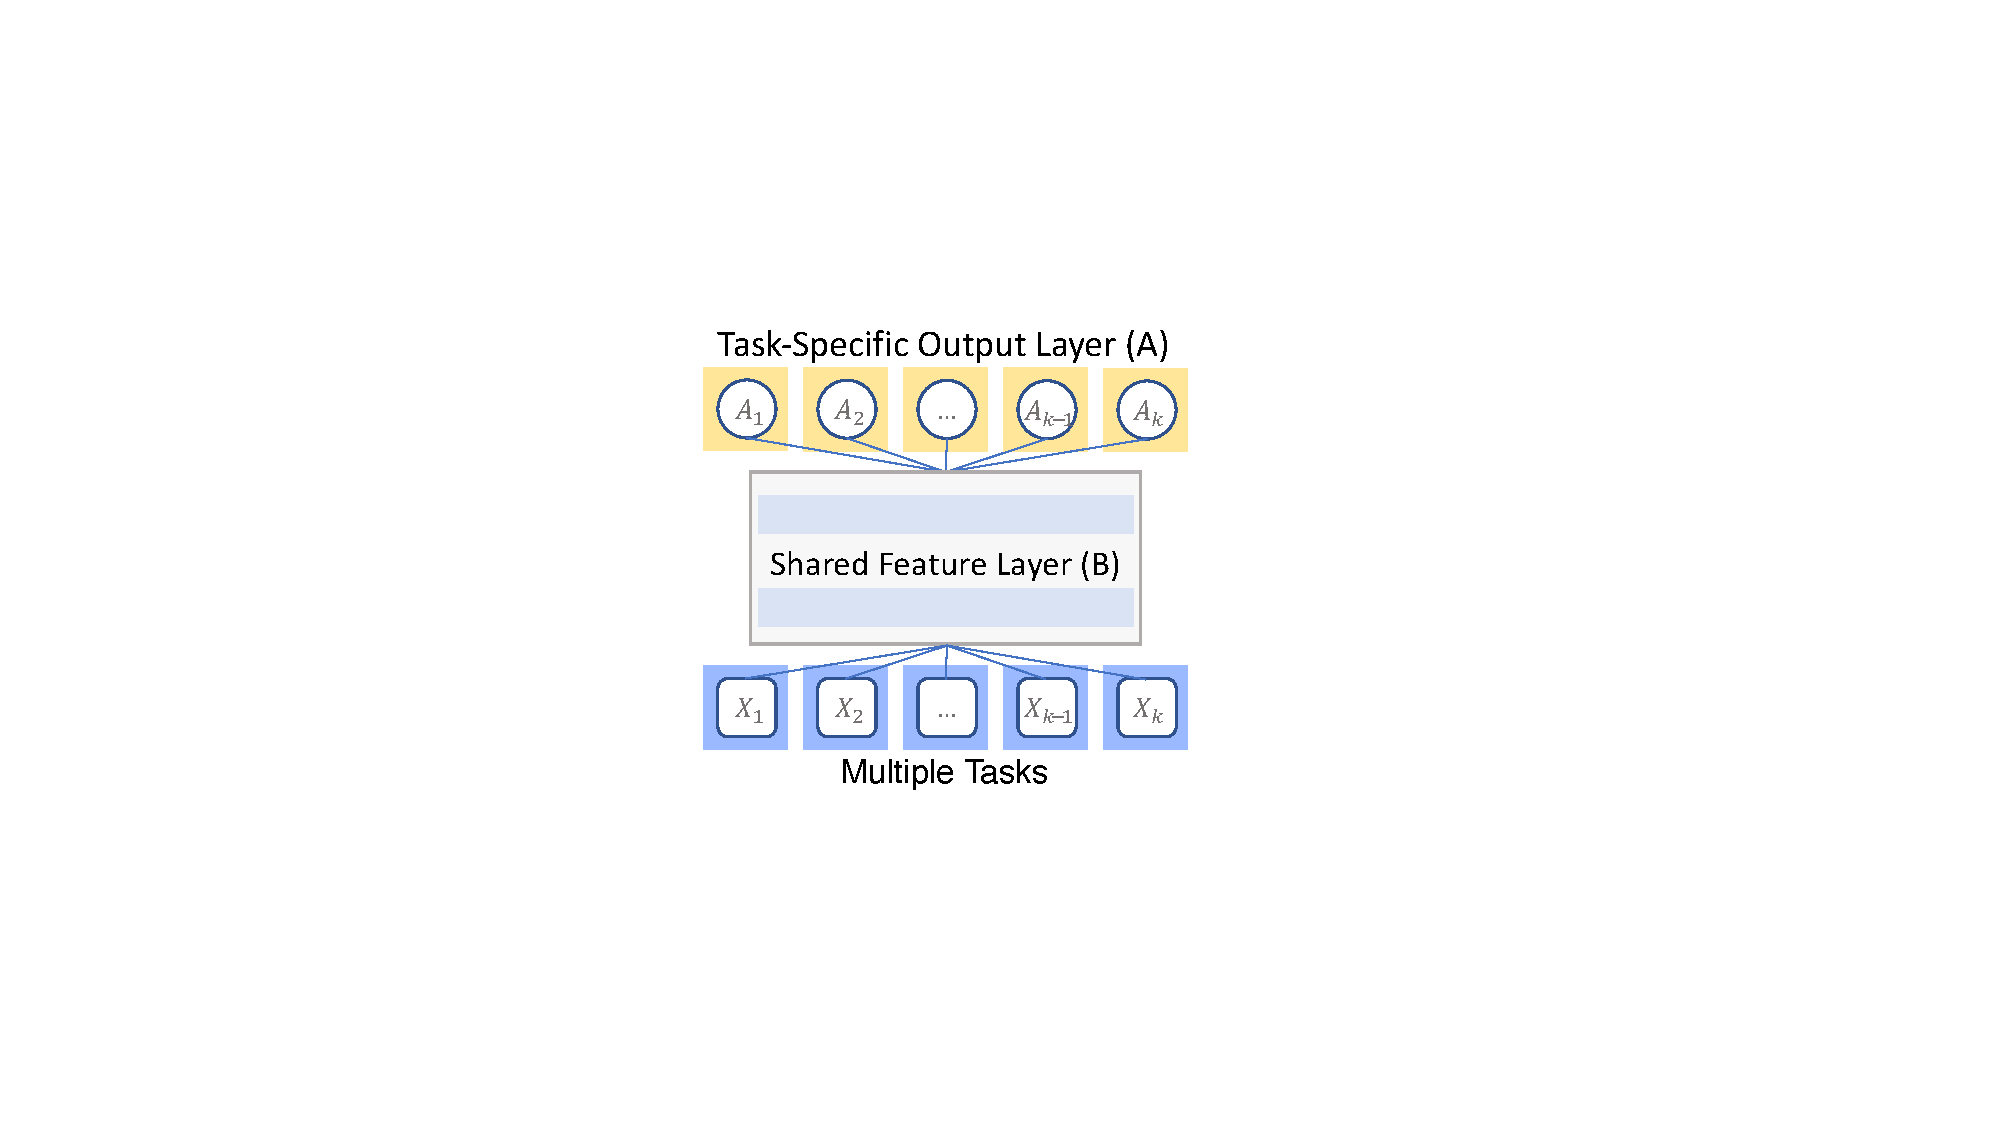
\includegraphics[width=0.45\textwidth,valign=t]{figures/mtl_model_arch.pdf}
		\caption{A hard parameter sharing architecture}
		\label{fig_intro_arch}
	\end{subfigure}\hfill
	\begin{subfigure}[t]{0.5\textwidth}
		\centering
		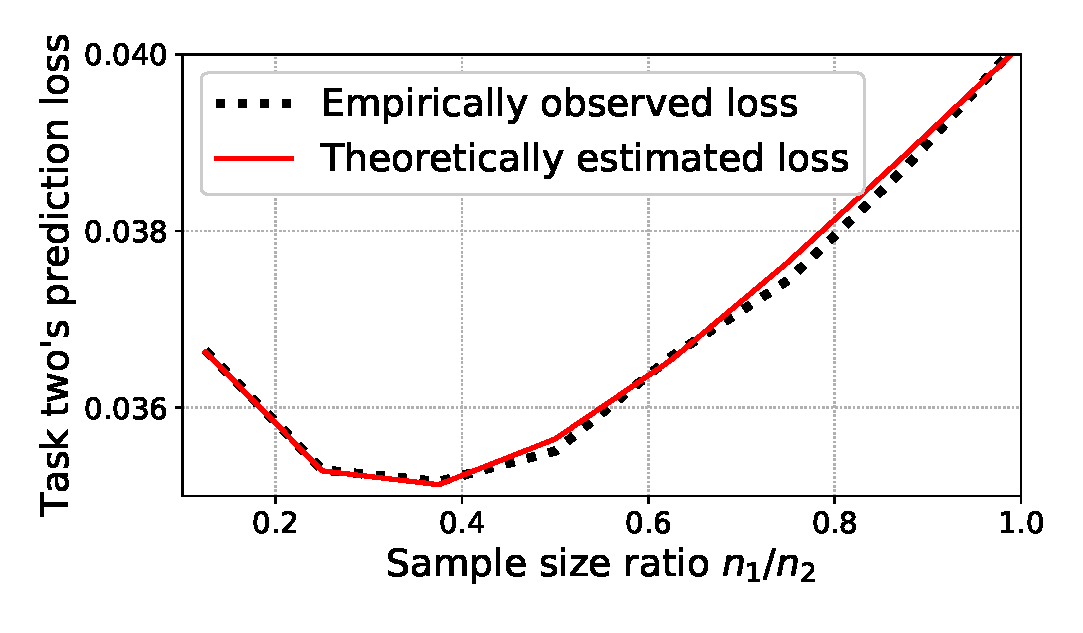
\includegraphics[width=0.745\textwidth,valign=t]{figures/sample_ratio_c2_400.eps}
		\caption{Varying sample size ratio}
		\label{fig_intro_sample_size_b}
	\end{subfigure}
	\vspace{-0.1in}
	\caption{
	Left: an illustrative picture of HPS.
	Right: an illustrative example of using HPS for two tasks $X_1, Y_1$ and $X_2, Y_2$ with sample size $n_1, n_2$, respectively.
	Increasing $n_1/n_2$ decreases task two's prediction loss initially but increase afterward. This phenomenon occurs due to different bias-variance tradeoffs as $n_1/n_2$ increases. Our result provides an estimated loss (solid line) that accurately matches the empirical loss (dotted line).
	See Section \ref{sec_simulation} for the precise setting.}
	\label{fig_intro_sample_size}
\end{figure*}



This paper presents new techniques to study hard parameter sharing and establishes a number of new results.
We consider regression analysis, which is arguably one of the most fundamental problems in statistics and machine learning.
We are interested in the \textit{high-dimensional} setting, where each dataset's sample size and feature dimension grow linearly instead of logarithmically.
This setting captures the fact that a single task's sample size is usually insufficient for accurate learning in many applications.
For example, if a dataset's sample size is only a constant factor of dimension in linear regression, the variance is also constant (cf. Fact \ref{fact_tr}).
The high-dimensional setting is challenging but is crucial for understanding how datasets' sample sizes impact generalization performance.

\subsection{Setup and definitions}
Consider the transfer learning setting with two data sets. We denote their sample sizes by $n_1$ and $n_2$. For $i=1,2,$ Let $X^{(i)} \in \real^{n_i \times p}$ denote dataset $i$'s feature covariates. We assume that the label vector $Y^{(i)} \in \real^{n_i}$ for $X^{(i)}$ follows a linear model plus random noise:
$$Y^{(i)}= X^{(i)}\beta^{(i)} + \varepsilon^{(i)},\quad i=1,2.$$
In this paper, we make the following assumptions on feature covariates $X^{(i)}$ and the noise vectors $\varepsilon^{(i)}$. We remark that all these assumptions are natural in high-dimensional statistics.

We assume that the row vectors of $X^{(i)}$ are i.i.d. centered random vectors with  population covariance matrix $\Sigma^{(i)}$. More precisely, let
\be\label{XofZ}X^{(i)} = Z^{(i)} (\Sigma^{(i)})^{1/2} \in \real^{n_i\times p},\quad i=1,2, \ee
where each $\Sigma^{(1)}$ and $\Sigma^{(2)}$ are $p\times p$ deterministic positive definite symmetric matrices, and $Z^{(1)}=(z^{(1)}_{ij})$ and $Z^{(2)}=(z^{(2)}_{ij})$ are $n_1\times p$ and $n_2\times p$ random matrices with real i.i.d. entries satisfying
\begin{equation}\label{assm1}
\mathbb{E} z^{(1)}_{ij}=\mathbb{E} z^{(2)}_{ij} =0, \ \quad \ \mathbb{E} \vert z^{(1)}_{ij} \vert^2=\mathbb{E} \vert z^{(2)}_{ij} \vert^2 =1,
\end{equation}

Another commonly used transfer learning estimator is defined as the minimizer of the total loss function \cite{bastani2020predicting, li2020transfer}:
$$\hat \beta^{\rm{TL}} := \argmin\left[ \norm{X^{(1)} \beta - Y^{(1)}}^2 + \norm{X^{(2)} \beta - Y^{(2)}}^2\right].$$

Given a solution from minimizing $f(A, B)$, denoted by $(\hat{A}, \hat{B})$  (which we will specify below), let $\hat{\beta}_i^{\MTL} = \hat{B} \hat{A}_i$ denote the HPS estimator for task $i$.
The critical questions are:
(i) How well does the estimator work? In particular, how does the performance of the estimator scale with sample size?
(ii) For datasets with different sample sizes and covariate shifts, how do they affect the estimator?


\subsection{Main results}
Our first result (Theorem \ref{thm_many_tasks}) applies to multi-label prediction settings where all datasets have the same features (and sample size), and we want to make several predictions for every input (cf. examples in \cite{hsu2009multi}).
We analyze the global minimizer of $f(A, B)$, and provide a sharp bias-variance decomposition of its (out-of-sample) prediction loss for any task.
This setting is tractable even though in general, $f(A, B)$ is non-convex in $A$ and $B$ (e.g. matrix completion is a special case for suitably designed $X^{(i)}, Y^{(i)}$).
%We show that the prediction loss of HPS admits a clean bias-variance decomposition.
Our result implies that when all tasks have the same features but different labels, for any task, HPS helps reduce the task's variance compared to single-task learning but increases bias.

Our second result (Theorem \ref{thm_main_RMT}) applies to two tasks with arbitrarily different sample size ratios and covariate shifts.
While we can no longer characterize $f(A, B)$'s global minimum because of non-convexity, we can still provide a sharp bias-variance tradeoff of any local minimizer's prediction loss for both tasks.
Despite being a simple setting, we observe several non-trivial phenomena by varying sample size ratios and covariate shifts between the two tasks.
See Figure \ref{fig_intro_sample_size_b} for an illustration of the former.
Consequently, using our precise loss estimates, we observe several qualitative properties of HPS for varying dataset properties.
\begin{itemize}
	\item \textit{Sample efficiency (Example \ref{ex_same_cov})}:
	One advantage of combining multiple datasets is that the requirement for labeled data reduces compared to single-task learning, a phenomenon that \cite{ZSSGM18} has observed empirically.
	Our results further imply that HPS's sample efficiency depends on model-specific variances across tasks vs. the noise variance and is generally high when the latter is large.

	\item \textit{Sample size ratio (Example \ref{ex_sample_ratio})}: Increasing one task's sample size does not always reduce another task's loss. In a simplified setting, we find that the task loss either decreases first before increasing afterward or decreases monotonically depending on how fast the bias grows. These two trends result from different bias-variance tradeoffs. This result is surprising because previous generalization bounds in multi-task learning typically scale down as all tasks' sample sizes increase, thus do not apply for different sample size ratios.

	\item \textit{Covariate shift (Example \ref{ex_covshift})}: In addition to sample sizes, variance also scales with two datasets' covariate shifts. For a large sample size ratio, HPS's  variance is smallest when there is no covariate shift. Counterintuitively, for a small sample size ratio, having covariate shifts reduces variance through a complementary spectrum. We achieve this result through a novel characterization on the inverse of the sum of two sample covariance matrices with arbitrary covariate shifts. See our discussion of proof techniques below for details.
\end{itemize}


Finally, we discuss the practical implications of our work.
Our sample size ratio study implies a concrete progressive training procedure that gradually adds more data until performance drops.
For example, in the setting of Figure \ref{fig_intro_sample_size_b}, this procedure will stop right at the minimum of the local basin.
We conduct further studies of this procedure on six text classification datasets and observe that it reduces the computational cost by $65\%$ compared to a standard round-robin training procedure while keeping the average accuracy of all tasks simultaneously.

\medskip
\noindent\textbf{Proof techniques.}
There are two main ideas in our analysis. The proof of our first result uses a geometric intuition that hard parameter sharing finds a ``rank-$r$'' approximation of the datasets.
We carefully keep track of the concentration error between the global minimizer of $f(A, B)$ and its population version (cf. equation \eqref{eq_A_star}).
The proof of our second result is significantly more involved because of different sample sizes and covariate shifts. We show that the inverse of the sum of two sample covariance matrices with arbitrary covariate shifts converges to a deterministic diagonal matrix asymptotically (cf. Theorem \ref{thm_main_RMT}).
We use recently developed techniques from random matrix theory to show a sharp convergence rate.
% to obtain a sharp estimate on the..., which is commonly referred to as the \emph{local law}.
%\HZ{add several sentences on the technical insight}
One limitation of our analysis is that in Example \ref{ex_sample_ratio}, there is an error term that can result in vacuous bounds for very small $n_1$ (cf. equation \eqref{cor_MTL_error}).
We believe our result has provided significant initial insights, and it is an interesting question to tighten our result.
See Section \ref{sec_conclude} for more discussions of the technical challenge.



\subsection{Related Work}

There is a large body of classical and recent works on multi-task learning.
We focus our discussion on theoretical results and refer interested readers to several excellent surveys for general references \cite{PY09,ZY17,V20}.
The early work of \cite{B00,BS03,M06} studied multi-task learning from a theoretical perspective, often using uniform convergence or Rademacher complexity based techniques.
An influential paper by \cite{BBCK10} provides uniform convergence bounds that combine multiple datasets in certain settings.
One limitation of uniform convergence based techniques is that the results often assume that all  tasks have the same sample size, see e.g. \cite{B00,MPR16}.
Moreover, these techniques do not apply to the high-dimensional setting because the results usually require a sample size of at least $p \log p$.

Our proof techniques use the so-called local law of random matrices \cite{erdos2017dynamical}, a recent development in the random matrix theory literature.
In the single-task case, \cite{isotropic} first proved such a local law for sample covariance matrices with isotropic covariance.
\cite{Anisotropic} later extended this result to arbitrary covariance matrices.
%On the other hand, one may derive the asymptotic result in Theorem \ref{thm_main_RMT} with error $\oo(1)$ using the free addition of two independent random matrices in  theory .
These techniques provide almost sharp convergence rates to the asymptotic limit compared to other methods such as free probability \cite{nica2006lectures}.
To the best of our knowledge, we are not aware of any previous results in the multi-task case, even for two tasks (with arbitrary covariate shifts).
\HZ{can you please add a discussion of the related work from RMT?}

The problem we study here is also related to high-dimensional prediction in transfer learning \cite{li2020transfer,bastani2020predicting} and distributed learning \cite{dobriban2018high}.
For example, \cite{li2020transfer} provide minimax-optimal rates to predict a target regression task given multiple sparse regression tasks.
One closely related work is \cite{WZR20}, which studied hard parameter sharing for two linear regression tasks.
However, their results only apply to sample size regimes at least logarithmic factors of dimension.
%\cite{WZR20} (and an earlier work by \cite{KD12}) observed that the shared layer size $r$ in hard parameter sharing plays a critical role of regularization.
%Linear models in multi-task learning have been studied in various settings, including online learning \cite{CCG10,DCSP18}, sparse regression \cite{LPTV09,LPVT11}, and representation learning \cite{BHKL19}.

%Our setting is closely related to domain adaptation \cite{DM06,BB07,BC08,DH09,MMR09,CWB11,ZS13,NB17,ZD19}.
%The important distinction is that we focus on predicting the target task using a hard parameter sharing model.
%For such models, their output dimension plays an important role of regularization \cite{KD12}.
%Below, we describe several lines of work that are most related to this work.

%Some of the earliest works on multi-task learning are Baxter , Ben-David and Schuller \cite{BS03}.
%Mauer \cite{M06} studies generalization bounds for linear separation settings of MTL.
%The benefit of learning multi-task representations has been studied for learning certain half-spaces \cite{MPR16} and sparse regression \cite{LPTV09,LPVT11}.
%Our work is closely related to Wu et al. \cite{WZR20}.
%While Wu et al. provide generalization bounds to show that adding more labeled helps learn the target task more accurately, their techniques cannot be used to explain when MTL outperforms STL.
%\todo{spell out the challenge more explicitly}

%Ando and Zhang \cite{AZ05} introduces an alternating minimization framework for learning multiple tasks.
%Argyriou et al. \cite{AEP08} present a convex algorithm which learns common sparse representations across a pool of related tasks.
%Evgeniou et al. \cite{EMP05} develop a framework for multi-task learning in the context of kernel methods.
%\cite{KD12} observed that controlling the capacity can outperform the implicit capacity control of adding regularization over $B$.
%The multi-task learning model that we have focused on uses the idea of hard parameter sharing \cite{C93,KD12,R17}.
%We believe that our theoretical framework can apply to other approaches to multi-task learning.



\subsection{Organizations}
The rest of this paper is organized as follows.
In Section \ref{sec_same}, we present the bias-variance decomposition for hard parameter sharing.
In Section \ref{sec_diff}, we describe how varying sample sizes and covariate shifts impact hard parameter sharing using random matrix theory.
In Sections \ref{sec_simulation}, we validate our results in simulations.
In Section \ref{sec_conclude}, we summarize our work and discuss future work.
Section \ref{sec_text} describes our study on text classification tasks.
Section \ref{app_proof_error_same_cov}, \ref{appendix RMT}, and \ref{app_iso_cov} present proofs of our results.
